\documentclass[11pt,a4paper]{article}
\usepackage[margin=2.5cm]{geometry}
\usepackage{amsmath}
\usepackage{graphicx}
\usepackage{booktabs}
\usepackage{float}
\usepackage{hyperref}

\title{Predicting Slow Leaders: Leadership Transfer against Gray Failures in Raft-based Distributed Systems}
\author{Raluca Boca}
\date{}

\begin{document}
\maketitle

\noindent Code and results: \url{https://github.com/bocaraluca/predictive-leader-transfer}

% =====================================================================
\section{Experimental Model}

In Raft~\cite{raft} all writes go through the leader, which sends them to the followers and waits for a majority to confirm. A follower starts a new election only when it stops receiving heartbeats from the leader. A leader that is slow but still alive keeps sending heartbeats, so it stays leader and the whole cluster becomes slow~\cite{grayfailure,onesize}.

The experiments answer the following question: \emph{can an external controller, which predicts from the trend of the leader latency that the leader is becoming slow and moves the leadership in advance, keep the write latency lower than a controller that only reacts after the slowdown is visible?} To answer it, the experiments measure how much the cluster suffers from a slow leader without any action, with a reactive controller and with a predictive controller, under the same conditions.

\subsection{Data}

No public dataset with measurements of slow Raft leaders was found, so all the data is produced by the experiments themselves, on a cluster where the slowdown is injected in a controlled way. Every run saves the following files:

\begin{itemize}
  \item \textbf{\texttt{workload.csv}} -- one row for every write: time, node that received it, duration in milliseconds and whether it succeeded. A client writes a key into etcd about 10 times per second, so a run of 140 seconds has around 1{,}000--1{,}400 writes. This is the latency that a user of the cluster sees, and all the metrics are computed from it.
  \item \textbf{\texttt{probes.csv}} -- once per second, the controller sends a status request to every node and saves the response time and which node is the leader. This is the only information the controller uses for its decisions; it does not read the write latency.
  \item \textbf{\texttt{actions.csv}} -- the decisions of the controller: the normal latency and the threshold learned at the start of the run, and every leadership transfer together with the values that triggered it.
  \item \textbf{\texttt{degrade.csv}} and \textbf{\texttt{meta.json}} -- the moments when each step of the slowdown was applied, and the start and end of the degradation, used to express all times relative to the start of the degradation.
\end{itemize}

Two separate measurements are used on purpose: the controller decides only from the status requests, which are cheap, while the evaluation uses the real write latency. In this way the controller is not evaluated on the same values it uses to decide.

\subsection{Environment and code}

\begin{itemize}
  \item \textbf{etcd 3.5.17} with 3 nodes. etcd is one of the most used Raft implementations (it stores the state of Kubernetes), it offers leadership transfer as a normal operation (\texttt{move-leader}, an extension of Raft described in~\cite{ongarothesis}) and it has an HTTP API that can be called directly from scripts.
  \item \textbf{Docker Compose} on one laptop (Windows, WSL2). Each node runs in its own container, so one node can be slowed down without affecting the others, and the whole cluster starts with one command.
  \item \textbf{tc netem} adds network delay to a node. It is run from a helper container that shares the network of the node. CPU limits are set with \texttt{docker update --cpus}.
  \item \textbf{Python} with \texttt{requests} for the etcd API and \texttt{pandas} and \texttt{matplotlib} for the analysis.
\end{itemize}

\begin{table}[H]
\centering
\small
\begin{tabular}{ll}
\toprule
Script & Role \\
\midrule
\texttt{workload.py}       & writes into etcd continuously and records the latency of every write \\
\texttt{common.py}         & node status, finding the leader, leadership transfer \\
\texttt{degrade.py}        & slows down a node according to a scenario \\
\texttt{controller.py}     & the controller, in mode \texttt{none}, \texttt{reactive} or \texttt{predictive} \\
\texttt{run\_experiment.py} & runs one complete experiment \\
\texttt{analyze.py}        & computes the metrics of all runs and draws the graphs \\
\bottomrule
\end{tabular}
\caption{The code used for the experiments.}
\end{table}

\subsection{Scenarios}

The slowdown is always applied to the leader. Before each run node \texttt{etcd1} is made leader, so the slowdown is always injected into the same node.

The case study uses the scenario \textbf{net-gradual}: the network delay of the leader grows step by step to 10, 20, 40, 60, 80, 100, 150 and 200\,ms, each step lasting 10 seconds, so the degradation lasts 80 seconds. It models a leader whose network or host gets worse slowly, which is the case where prediction should help most.

The code also supports a sudden delay (\texttt{net-sudden}), gradual and sudden CPU limits, and a scenario with only short random spikes of delay (\texttt{spikes}). The last one contains no real slowdown and will be used to count false alarms during the validation. CPU limits are not used in the case study, because the motivation experiment (Section~\ref{sec:motivation}) showed that they have no visible effect in this environment.

\subsection{Compared variants}

Three variants are compared in every scenario:
\begin{itemize}
  \item \textbf{none} -- the controller only measures and never acts. This is the default behaviour of etcd and shows how large the problem is.
  \item \textbf{reactive} -- the leadership is moved after the leader has been above a threshold for 5 seconds in a row. This represents the existing approaches, which detect a slow node after the slowdown has appeared~\cite{iaso,perseus}.
  \item \textbf{predictive} -- the leadership is moved when the trend of the leader latency predicts that it will cross the threshold within the next 10 seconds. This is the proposed approach.
\end{itemize}
The two active variants use the same threshold, the same rule for choosing the new leader and the same transfer mechanism. The only difference is the moment when they decide to act, so any difference in the results comes from the prediction.

\subsection{Mathematical model}

Let $r_i(t)$ be the response time of node $i$ to the status request at second $t$, and $L$ the current leader.

\paragraph{Smoothing.} A single slow response should not trigger anything, so the leader latency is smoothed with a median over the last three seconds:
\begin{equation}
  s(t) = \operatorname{median}\big(r_L(t-2),\, r_L(t-1),\, r_L(t)\big).
\end{equation}

\paragraph{Learning phase.} In the first $T_\ell = 15$ seconds the controller does not act. It learns the normal latency $\mu$ of the leader and computes the threshold $\theta$ above which the leader is considered slow:
\begin{equation}
  \mu = \operatorname{median}\{\, s(t) : t < T_\ell \,\}, \qquad
  \theta = \max\big(k\mu,\; \mu + m\big), \quad k = 3,\; m = 20\,\text{ms}.
\end{equation}
The threshold is three times the normal latency, but at least 20\,ms above it, so that a very low normal latency does not give a threshold that is too close to the noise. For example, $\mu = 15$\,ms gives $\theta = \max(45, 35) = 45$\,ms.

\paragraph{Reactive rule.} The leadership is moved at second $t$ if the leader was above the threshold for the last $K = 5$ seconds:
\begin{equation}
  s(t-j) > \theta \quad \text{for all } j = 0, 1, \dots, K-1.
\end{equation}

\paragraph{Predictive rule.} The trend of the leader latency is the slope of the least-squares line through the last $W = 10$ smoothed values $s_x = s(t-W+1+x)$, $x = 0, \dots, W-1$:
\begin{equation}
  \beta(t) = \frac{\sum_{x=0}^{W-1} (x - \bar{x})(s_x - \bar{s})}{\sum_{x=0}^{W-1} (x - \bar{x})^2},
\end{equation}
where $\bar{x}$ and $\bar{s}$ are the means of $x$ and $s_x$. The slope says by how many milliseconds the latency grows each second. The latency expected $H = 10$ seconds later is the current level (the mean of the last three values) plus the slope multiplied by $H$:
\begin{equation}
  \hat{s}(t+H) = \frac{1}{3}\sum_{j=0}^{2} s(t-j) + \beta(t)\, H.
\end{equation}
An alarm is raised when $\hat{s}(t+H) > \theta$, and the leadership is moved after two consecutive alarms, which reduces the effect of noise. For example, if the current level is 22\,ms and the latency grows by 2\,ms per second, the prediction is $22 + 2 \cdot 10 = 42$\,ms; with a threshold of 40\,ms the controller acts now, before the leader actually reaches the threshold.

\paragraph{New leader and cooldown.} The new leader is the follower with the lowest median response time in the last five seconds,
\begin{equation}
  L' = \arg\min_{j \neq L} \operatorname{median}\{\, r_j(t-4), \dots, r_j(t) \,\},
\end{equation}
and after a transfer no other transfer is allowed for $C = 30$ seconds, so that the leadership is not moved back and forth.

\subsection{Metrics}

All metrics are computed from the write latency after the start of the degradation ($t \ge 0$):
\begin{itemize}
  \item \textbf{median} and \textbf{p99 latency} -- the typical and the tail latency seen by the client. The tail matters because in distributed systems the slowest requests decide the user experience~\cite{tailatscale};
  \item \textbf{slow seconds} -- the number of seconds in which the median write latency is more than twice the normal latency (the median before the degradation);
  \item \textbf{transfers} -- the number of leadership transfers; a transfer before $t = 0$ is a false alarm;
  \item \textbf{first transfer} $T$ -- how many seconds after the start of the degradation the controller acted, and the \textbf{lead time} $T_{\text{reactive}} - T_{\text{predictive}}$, which shows how much earlier the predictive variant reacts.
\end{itemize}

\subsection{Experimental procedure and validation}

Every run is executed by one script (\texttt{run\_experiment.py}), always with the same steps:
\begin{enumerate}
  \item all slowdowns are removed from all nodes;
  \item \texttt{etcd1} is made leader;
  \item the workload and the controller are started; the workload sends writes only to the two followers, so the client never talks directly to the node that will be slowed down;
  \item the cluster runs normally for 30 seconds (the controller uses the first 15 for the learning phase);
  \item the degradation is applied to \texttt{etcd1} for 80 seconds and then removed;
  \item the cluster runs for another 30 seconds and the run ends.
\end{enumerate}

To make the results trustworthy, all variants run under the same conditions, every combination of scenario and variant is repeated three times, and the parameters of the controller ($T_\ell$, $k$, $m$, $K$, $W$, $H$, $C$) were fixed before the experiments and were not changed after seeing the results. The predictive variant is considered better if it acts earlier than the reactive one, with a lower or equal tail latency and without more false alarms.

% =====================================================================
\section{Case Study}

This chapter applies the model to a small initial set of experiments: two motivation experiments without any controller and nine runs of the \texttt{net-gradual} scenario.

\subsection{Motivation: does a slow leader matter?}
\label{sec:motivation}

Before building the controller, the effect of a slow leader was measured without any action. The workload ran for 60 seconds and after about 20 seconds the leader was slowed down.

\begin{table}[H]
\centering
\begin{tabular}{lcccc}
\toprule
Slowdown on the leader & Before (ms) & After (ms) & Writes / minute & Leader changed \\
\midrule
CPU limited to 10\%     & 57.5 & 57.6  & --  & no \\
Network delay 100\,ms   & 49.2 & 208.4 & 606 $\rightarrow$ 360 & no \\
\bottomrule
\end{tabular}
\caption{Median write latency before and after slowing down the leader, without any controller.}
\end{table}

Limiting the CPU to 10\% of a core had no effect. etcd does very little computation for a write, and in this environment most of the time of a write is spent waiting for the disk (WSL2), so the CPU limit is hidden by the disk time.

The network delay had a large effect. The median latency grew from 49.2 to 208.4\,ms, about 160\,ms more, and since the client waits for each write, the number of writes in one minute dropped from 606 to 360. The latency grew by much more than 100\,ms because a write passes through the delayed leader twice: the follower forwards the request to the leader, whose answer is delayed, and the leader sends the new entry to the followers, which is delayed as well. During all this time the leader did not change and the Raft term stayed the same, so etcd treated the slow leader as healthy. This is the behaviour described in~\cite{onesize} and shows that an external mechanism is needed.

\subsection{Setup}

The case study uses \texttt{net-gradual} with the three variants and three repetitions each, so nine runs of 140 seconds (30\,s normal, 80\,s degradation, 30\,s after). The controller parameters are the ones from the model: $T_\ell = 15$\,s, $k = 3$, $m = 20$\,ms, $K = 5$, $W = 10$, $H = 10$\,s and $C = 30$\,s.

\subsection{Results}

\begin{table}[H]
\centering
\small
\begin{tabular}{lcccccc}
\toprule
Run & Normal (ms) & Median (ms) & p99 (ms) & Slow s & Transfers & First tr. (s) \\
\midrule
none, rep 1       & 49.0 & 53.7 & 424.8 & 51 & 0 & -- \\
none, rep 2       & 49.3 & 56.8 & 427.9 & 51 & 0 & -- \\
none, rep 3       & 52.5 & 67.0 & 412.7 & 52 & 0 & -- \\
reactive, rep 1   & 49.1 & 49.2 & 70.5  & 0  & 1 & 8.5 \\
reactive, rep 2   & 49.6 & 49.3 & 88.0  & 0  & 1 & 26.6 \\
reactive, rep 3   & 53.4 & 54.8 & 93.9  & 0  & 1 & 26.8 \\
predictive, rep 1 & 48.9 & 49.2 & 64.6  & 0  & 1 & $-12.6$ \\
predictive, rep 2 & 56.7 & 53.0 & 79.0  & 0  & 1 & 4.6 \\
predictive, rep 3 & 58.0 & 54.7 & 80.5  & 0  & 1 & 14.8 \\
\midrule
none, average       & -- & 59.2 & 421.8 & 51.3 & 0 & -- \\
reactive, average   & -- & 51.1 & 84.1  & 0    & 1 & 20.6 \\
predictive, average & -- & 52.3 & 74.7  & 0    & 1 & 9.7\textsuperscript{*} \\
\bottomrule
\end{tabular}
\caption{Results of the nine runs and averages per variant. Times are relative to the start of the degradation. \textsuperscript{*}Repetitions 2 and 3 only; in repetition 1 the transfer was a false alarm (Section~\ref{sec:limits}).}
\label{tab:runs}
\end{table}

\begin{figure}[H]
\centering
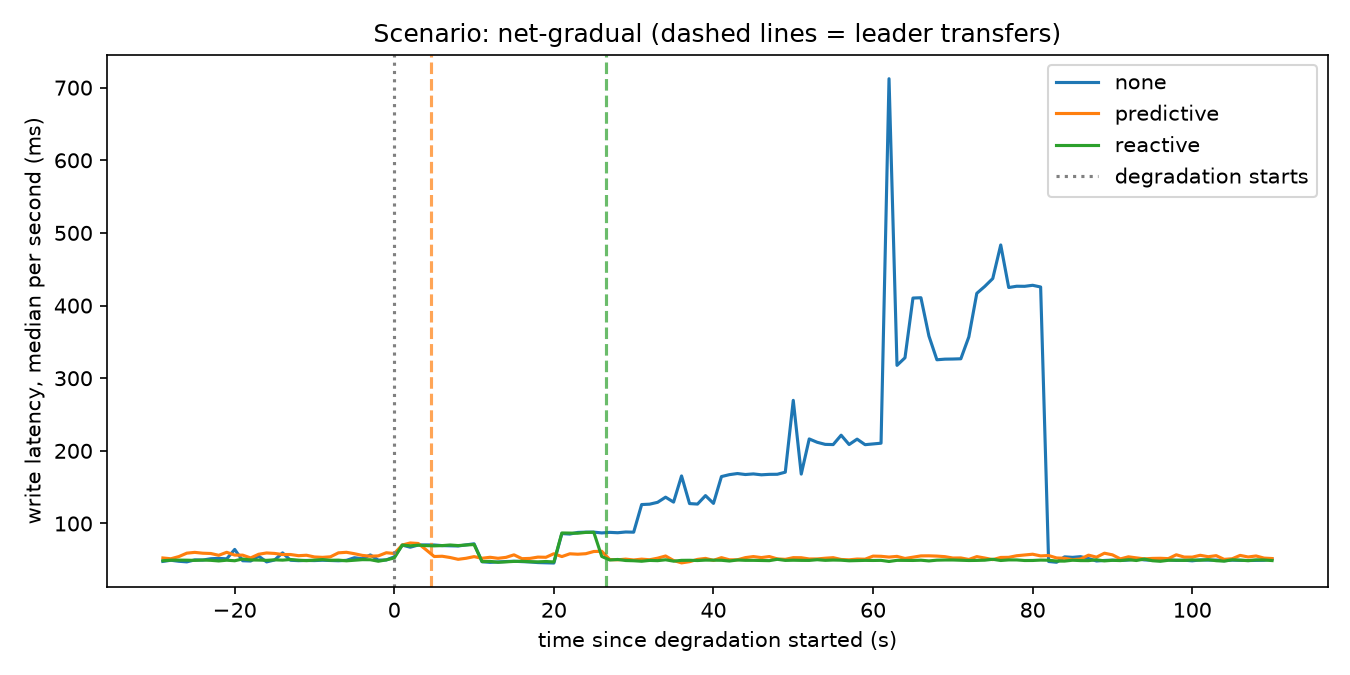
\includegraphics[width=0.72\linewidth]{latency_rep2.png}
\caption{Write latency (median per second) in repetition 2. The dotted line is the start of the degradation and the dashed lines are the leadership transfers of each variant.}
\label{fig:rep2}
\end{figure}

\subsection{Interpretation}

\paragraph{The problem without a controller.} In the variant \texttt{none} the latency follows the steps of the degradation and reaches more than 400\,ms at the end (Figure~\ref{fig:rep2}, blue line). The cluster is slow for about 51 of the 80 seconds of degradation and the p99 latency is above 410\,ms in all three runs. The leader never changes, which confirms the motivation experiment on a longer and gradual slowdown.

\paragraph{Both controllers solve the problem.} With either controller there are no slow seconds left and the p99 latency drops from about 420\,ms to under 95\,ms. Every run has exactly one transfer, so the cooldown works and the leadership does not move back and forth. After the transfer the latency returns to its normal value, because the slow node is now a follower and a majority can be formed without waiting for it.

\paragraph{Predictive compared to reactive.} In the two valid runs, the predictive controller moved the leadership at 4.6 and 14.8 seconds after the start of the degradation, while the reactive one did it at 26.6 and 26.8 seconds, so the lead time was 22.0 and 12.0 seconds. Figure~\ref{fig:rep2} shows what this means for the client: the reactive variant (green) stays on the slow leader for two steps of the degradation, at about 70\,ms and then about 87\,ms, while the predictive variant (orange) leaves it after the first step. The average p99 latency is 74.7\,ms for the predictive variant (79.8\,ms if only the valid runs are counted) and 84.1\,ms for the reactive one. In repetition 1 the reactive controller acted earlier than usual (8.5\,s), which shows that the moment of the reaction also depends on the noise during the learning phase.

\paragraph{Conclusion of the case study.} The initial results support the approach: a slow leader that etcd keeps can be moved by an external controller without changing etcd, and predicting the trend makes the controller act clearly earlier than waiting for several slow seconds. Because the degradation is gradual, the leader is still only slightly slow when the reactive controller acts, so the difference in latency between the two controllers is small, while the difference in reaction time is large. The main weakness is the false alarm described below.

\subsection{Limitations}
\label{sec:limits}

\paragraph{False alarm.} In repetition 1 the predictive controller moved the leadership 12.6 seconds before the degradation started (Figure~\ref{fig:rep1}). The learning phase measured an unusually low normal latency, 8.38\,ms instead of about 15\,ms in the other runs, so the threshold was only 28.38\,ms. The status requests normally vary between 5 and 30\,ms, so this threshold was inside the normal noise. Two seconds after the learning phase, a spike of 23.2\,ms produced a positive slope and a predicted value of 41.4\,ms, which triggered the transfer. After that \texttt{etcd1} was no longer the leader, so the degradation did not affect the cluster in that run. The cause is that the threshold uses only the median of the learning phase and ignores how much the latency varies.

\begin{figure}[H]
\centering
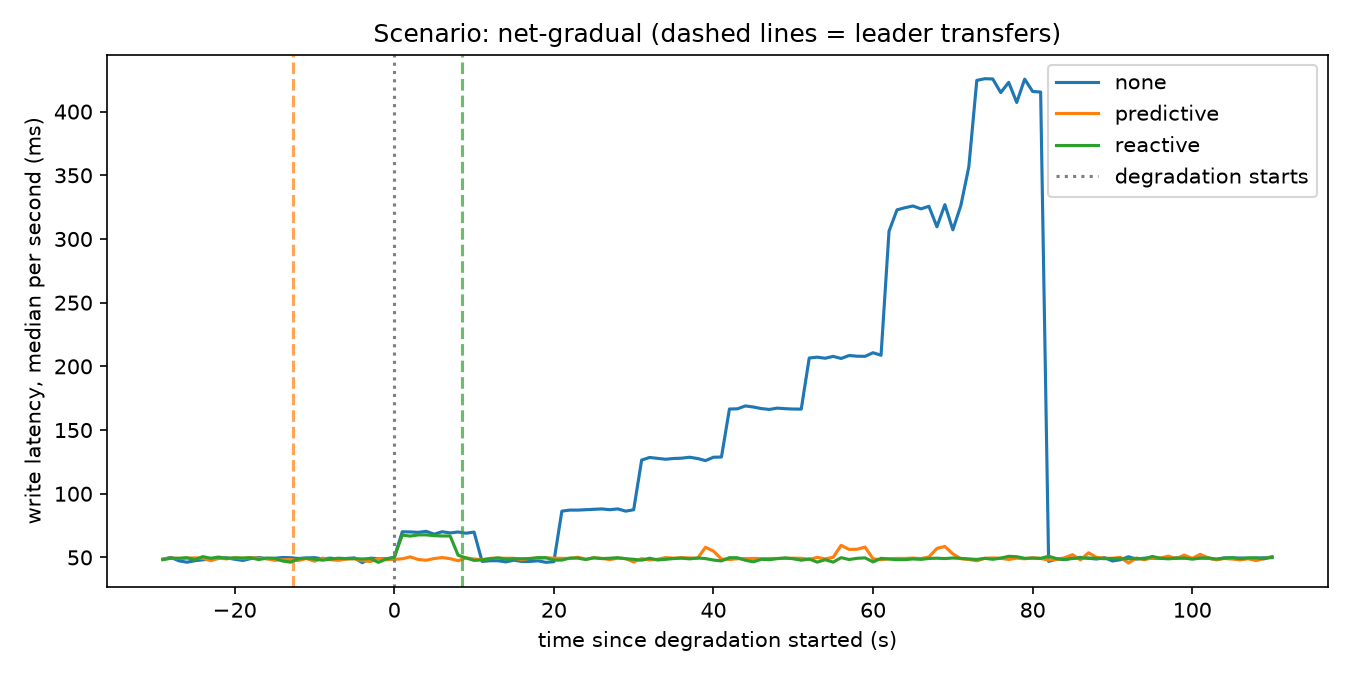
\includegraphics[width=0.72\linewidth]{latency_rep1.png}
\caption{Repetition 1: the predictive controller moves the leadership before the degradation starts (false alarm).}
\label{fig:rep1}
\end{figure}

\paragraph{Other limitations.}
\begin{itemize}
  \item Everything runs on one laptop. The normal write latency is about 50\,ms because of the slow disk access in WSL2, much higher than on a real server, and the three nodes share the same machine.
  \item Only one scenario and three repetitions were run, and the predictive variant has only two valid runs, so the averages are not yet reliable.
\end{itemize}

% =====================================================================
\section{Related Work}

This chapter presents the approaches from the literature that are closest to this work, the similarities and differences, the plan for validating the results and the metrics where similar or better results are expected.

\subsection{Slow and gray failures}

Huang et al.~\cite{grayfailure} introduce the term \emph{gray failure} for failures that the failure detector of a system does not see, but its users do, and show that they cause many incidents in cloud systems. Gunawi et al.~\cite{failslow} analyse more than one hundred reports from large production systems and show that \emph{fail-slow} components, which still work but much slower than normal, are common and can slow down a whole cluster. Lu et al.~\cite{onesize} study how six distributed systems, including etcd, react to slow components and show that a slightly slow leader is not replaced, because it still answers heartbeats. Jensen et al.~\cite{raftpartial} show that Raft can also lose availability during partial network failures. These works describe the problem; the motivation experiment of this report reproduces it on etcd.

\subsection{Reactive detection and mitigation}

IASO~\cite{iaso} detects slow nodes in a distributed storage system from the timeouts reported by their peers and isolates them; when the slow node is the leader of ZooKeeper, it restarts it so that a new leader is elected. Perseus~\cite{perseus} detects slow disks in a large cloud storage system by comparing their latency with the latency that is normal for the current load.

\emph{Similarities:} like these systems, this work watches the latency of the nodes from the outside and decides from a threshold learned from normal behaviour; the reactive variant of the controller follows the same principle. \emph{Differences:} these systems act after the slowdown has appeared, while the predictive controller acts before it becomes large, and it moves the leadership instead of restarting the node, so no node is lost.

\subsection{Slowdown-tolerant consensus}

Copilots~\cite{copilots} changes the replication protocol so that two leaders work in parallel and the system stays fast if one of them is slow. Avicenna~\cite{avicenna} compares the current leader with what a backup leader would have done and replaces the leader quickly when it is slow. SEER~\cite{seer} changes the leader election of a single-leader protocol so that the leader is chosen by its performance.

\emph{Similarities:} they solve the same problem, a slow leader in a consensus protocol. \emph{Differences:} they all require changes to the consensus protocol, so they cannot be used on an existing etcd cluster. This work does not modify etcd and only uses the leadership transfer it already offers~\cite{ongarothesis}.

\subsection{Failure prediction}

UBL~\cite{ubl} learns the normal behaviour of virtual machines without labels and predicts performance anomalies before they happen. Lin et al.~\cite{nodefailure} predict which nodes of a cloud service will fail, and Xu et al.~\cite{diskerror} predict disk errors, so that virtual machines can be moved away in advance.

\emph{Similarities:} the idea of predicting a problem and acting before it happens. \emph{Differences:} these works predict failures of whole machines or disks and act by moving virtual machines, which takes minutes, while this work predicts the slowdown of the Raft leader and acts by a leadership transfer, which takes less than a second.

\subsection{Comparison}

\begin{table}[H]
\centering
\small
\begin{tabular}{lcccc}
\toprule
Approach & When it acts & Changes protocol & Restarts nodes & Unmodified etcd \\
\midrule
IASO~\cite{iaso}         & after slowdown  & no  & yes & no  \\
Perseus~\cite{perseus}   & after slowdown  & no  & no  & no  \\
Copilots~\cite{copilots} & always          & yes & no  & no  \\
Avicenna~\cite{avicenna} & after slowdown  & yes & no  & no  \\
SEER~\cite{seer}         & at election     & yes & no  & no  \\
This work                & before slowdown & no  & no  & yes \\
\bottomrule
\end{tabular}
\caption{Comparison with the closest approaches.}
\end{table}

\subsection{Validation plan}

There is no public dataset of slow Raft leaders, so the validation will use the same kind of slow-fault injection as~\cite{onesize}, which also slows down the network and the CPU of the etcd leader. In this way the behaviour with and without a controller can be compared with the one reported there. Compared to the case study, the validation will add:
\begin{itemize}
  \item the \texttt{net-sudden} and \texttt{spikes} scenarios, to measure the behaviour for sudden slowdowns and the number of false alarms;
  \item five repetitions per variant instead of three;
  \item a threshold that also takes into account the variance measured in the learning phase, to avoid the false alarm seen in the case study;
  \item a second predictor based on logistic regression, compared with the linear trend.
\end{itemize}

\subsection{Expected results}

Compared to the literature, the expected results are:
\begin{itemize}
  \item \textbf{better} reaction time and p99 latency than the reactive approaches (IASO, Perseus) for gradual slowdowns -- the case study already shows a lead time of 12--22 seconds and a lower p99 than the reactive variant;
  \item \textbf{better} applicability than Copilots, Avicenna and SEER, since etcd is not modified and no node is restarted;
  \item \textbf{similar} results to the reactive approach for sudden slowdowns, where there is no trend to predict;
  \item \textbf{worse} results in the number of false alarms, since a prediction from a trend can react to noise; this is the main point to improve in the validation.
\end{itemize}

% =====================================================================
\bibliographystyle{acm}
\bibliography{refs}

\end{document}